\renewcommand{\theequation}{\theenumi}
\renewcommand{\thefigure}{\theenumi}
\begin{enumerate}[label=\thesubsection.\arabic*.,ref=\thesubsection.\theenumi]
\numberwithin{equation}{enumi}
\numberwithin{figure}{enumi}

\item The coordinates of the vertices of a triangle are $(x_1,y_1)$, $(x_2,y_2)$ and $(x_3,y_3)$. The line joining the first two is divided in the ratio $l:k$, and the line joining his point of division to the opposite angular point is then divided in the ratio  $m:k+l$. Find the coordinates of the latter point of section. 
%
\\
\solution
From elementary analysis of coordinate geometry and in view of Fig.\ref{eq:solutions/2/22/f2}, as $\bf{D}$ divides the line AB in the ratio $AD:DC=l:k$, we have:

\begin{equation}
 {\bf{D}}=\frac{l{\bf{B}}+k\bf{A}}{l+k}
    \label{eq:solutions/2/22/eq4}
\end{equation}
The position vector $\bf{E}$ which  divides CD in the ratio $DE:EC=m:l+k$,  is clearly obtained by setting $l=m,k=l+k,\bf{A=D,B=C}$ and is given by: 

\begin{equation}
 {\bf{E}}=\frac{m{\bf{C}}+(l+k)\bf{D}}{m+l+k}
    \label{eq:solutions/2/22/eq5}
\end{equation}
 
Using Eq.\ref{eq:solutions/2/22/eq4} into Eq.\ref{eq:solutions/2/22/eq5} and simplifying yields :
\begin{equation}
 {\bf{E}}=\frac{m {\bf{C}}+l{\bf{B}}+k{\bf{A}}}{m+l+k}
    \label{eq:solutions/2/22/eq6}
\end{equation}

Where,
%\begin{align}
 $  \bf{A}  = \begin{pmatrix}
           x_{1} \\
           y_{1} \\
         \end{pmatrix}$, $ \bf{B}  = \begin{pmatrix}
           x_{2} \\
           y_{2} \\
         \end{pmatrix}$  and $  \bf{C}  = \begin{pmatrix}
           x_{3} \\
           y_{3} \\
         \end{pmatrix}$
         
In Fig.\ref{eq:solutions/2/22/f2}, the solution obtained from the Python code is depicted for a particular choice of input viz. $l=1,m=1,k=1$ and $A(0,0),B(3,3)\, $\&$\, C(6,0)$.
Using, Eq.\ref{eq:solutions/2/22/eq6} and the above mentioned input, we have:

$  \bf{E}  = \begin{pmatrix}
           x_{E} \\
           y_{E} \\
         \end{pmatrix}$ $=\begin{pmatrix}
           3 \\
           1 \\
         \end{pmatrix}$



 \begin{figure}[!ht]
    \centering
    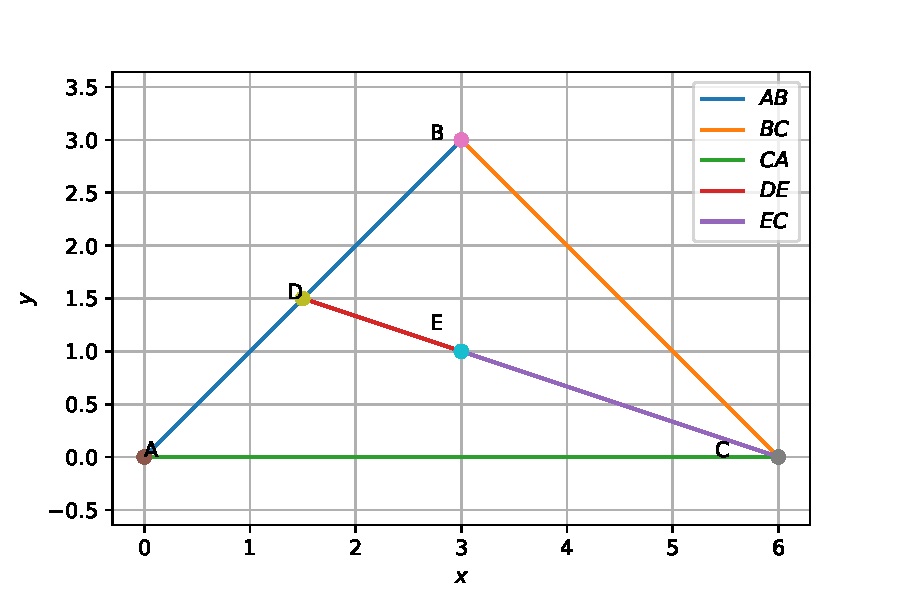
\includegraphics[width=\columnwidth]{./solutions/2/22/Ex1prob22.pdf}
    \caption{For $l=1,m=1,k=1$ and $A(0,0),B(3,3)\, $\&$\, C(6,0)$, the solution $E(3,1)$ is obtained using Python}
    \label{eq:solutions/2/22/f2}
\end{figure}
       


\end{enumerate}
